%!TEX root = ../dissertation.tex

\iffalse \bibliography{bibliography/dissertation} \fi

\chapter{Designing a Programming Environment for Generative Design}
\label{chapter:pegd}

This chapter presents the design of a coherent system integrating the previously studied techniques for interactive programming. The first part discusses the importance of good design principles in software engineering, highlighting the lack of tools that enforce those principles in the current programming systems, especially in the Architecture area where programming methods are increasingly popular. The second part introduces concrete tools for documenting a program and proposes a framework for providing immediate feedback as the developer write his code. While the following chapter discusses technical aspects and the software architecture, this chapter elaborates on the rationale behind all design decisions.

\section{Design Principles: a recurring need} 

Programming is hard to learn. Unfortunately, as shown in the previous sections, few programming languages or environments are intended to introduce the basics of good software engineering practice. Especially in Architecture, the environments used to support \gls{gd} either they are old or obsolete, or they enforce particular programming methods that are inadequate, or they are not pedagogic, meaning that they are not designed for the specific programming skills of the \gls{gd} community.

The literature in this area is vast, but it is clearly divided into two perspectives: \textit{software engineering perspective}, or \textit{psychological/educational perspective}. Which means that systems are either designed for expert programmers~\citep{carlson2005eclipse,intellij2001intellij,lighttable,boudreau2002netbeans,guckenheimer2006software}, or for novices programmers~\citep{papert1980mindstorms,goldberg1983smalltalk,GuoSIGCSE2013,Reas2006}. However, in the set of systems presented in Chapter~\ref{chapter:relatedWork}, is very unlikely a system that implements these two perspectives, allowing users to evolve their knowledge about programming gradually, without having to change to another environment. Even worst, the systems designed for novices usually offer a reduced set of programming tools, which consequently restricts the use of many other tools potentially useful. 

This problem becomes especially severe in the category of empowering systems because these systems would encourage novice programmers to evolve, enforcing the good practices of software engineering. Unfortunately, in the majority of systems presented in the previous sections, this rarely happens. For example, in Architecture area, due to the increasing adoption of \gls{gd} methods, and eventually the increasing complexity of \gls{gd} programs, the implementation of a programming system that preserve these good principles becomes crucial.

In the next sections, I discuss some design principles that improve program comprehension and also program documentation. Most of these principles were the congruous contributions that, unfortunately, are vaguely represented in current systems, mainly considering the methods used in \gls{gd} area. For that reason, I propose a generic implementation of a modern programming environment that meets the \gls{gd} community needs.

\section{Program Documentation}

Program documentation is a software requirement of the utmost importance because it is an essential factor for understanding programs. Even the best program, the most perfectly suitable for the job, will be mostly useless if the people who need to use it do not know what it is; cannot understand it well enough to use, build, or modify it; or (worst of all) misunderstand it and apply it incorrectly. This means that all of the effort, analysis, hard work, and insightful design spend to construct it will have been wasted.

Software exists for a particular reason, and documentation exists to explain this reason. Every piece of code has its rational and a reason to be written in that way. Then, the documentation collects all these rationales organizing them in a form of different artifacts, such as requirements description, architectural models, data models, \gls{api} documentation, flow diagrams, use case diagrams, etc. Therefore, it is, undoubtedly, a wealthy source of information not only for the developer who did the software, but also for the developer who will test the application, for the stakeholder who will use the application, and eventually for the developer who will maintain that code.

In fact, software maintenance is traditionally defined as any modification made on a system after its delivery; this is a dominant activity in software engineering. Some reports place maintenance at 90\% of the total cost of a typical software project~\citep{seacord2003modernizing,pigoski1996practical}. One of the main difficulties in software maintenance is a lack of up-to-date documentation~\citep{de2005study}. As a result, some studies indicate that 40\% to 60\% of maintenance activity is spent only studying existing software~\citep[p. 475 and p. 35 respectively]{pigoski1996practical,pfleeger1998software}. Having an updated documentation would dramatically reduce the effort spent in this study, helping the developer to comprehend the code and maintain it.

Unfortunately, the sad truth is that writing program documentation today is perceived as a tiresome task, if it is done at all, is often treated as an afterthought, something people do because they have to~\citep{sousa1998survey}. Bass et al. summarizes many possible reasons that lead programmers to write the documentation, and then concluded as follows:

\blockquote{Maybe a contract requires it. Maybe a customer demands it. Maybe a company's standard process calls for it. In fact, these may all be legitimate reasons. But none of them are compelling enough to produce high-quality documentation.~\citep[p. 327]{BassClementsKazman201210}}

Providing a high-quality documentation should be a natural developer's attitude not because it's ``required" but because they see that it is essential to the matter at hand. The documentation defends the developer's job because it speaks for him, for example in agile methods it can be used as a contract~\citep{ambler2007agile}. It also helps developers reason about the architecture design of their programs and communicates these ideas while the development is in progress. However, producing useful documentation is a hard task and developers have to consider that some documentation artifacts are more important than others, where each artifact is intended to communicate information on the software system~\citep{forward2002relevance}. This communication is aimed at human readers, from the technical document delivered to the developer team, up to the user manual provided to the users. But the central point from where the documentation comes from is the source code. As a result, the source code is the most valuable artifact, as suggested in the following study:

\blockquote{Source code and comments are the most important artifact to understand a system to be maintained. Data model and requirement description were other important artifacts. Surprisingly, and contrary to what we found in the literature, architectural models and
other general view of the system are not very important. This could simply indicate that such documentation artifacts are used once to have a global understanding of the system and never consulted again after.~\citep[p. 74]{de2005study}}

\subsection{Tools for documenting software programs}
\label{subsec:generalprograms}

The importance of source code and comments is a reality already noted in the software industry. Consequently, the use of automation tools to generate, verify, and maintain the source code documentation, is a notorious practice. The most frequently cited technologies, as concluded in~\citep{forward2002relevance}, are Javadoc\footnote{\texttt{http://docs.oracle.com/javase/7/docs/technotes/guides/javadoc/}}, and DocWiz\footnote{\texttt{http://docwiz.sourceforge.net/}} to comment Java source code, and Doc++\footnote{\texttt{http://docpp.sourceforge.net/}} and Doxygen\footnote{\texttt{http://www.stack.nl/dimitri/doxygen/index.html}} to comment source code in languages such as C, C++, and also Java. These tools generate the documentation from a set of documented source files into the selected format; the most commons are HTML, and $\mbox{\LaTeX}$. The comments are inserted directly in the source code between a start tag and an end tag. Typically, these tags use the language's comment delimiter to avoid compilation errors, as the compiler ignores any word between comment delimiters. For example, Javadoc requires an extra asterisk, when compared with C standard comments (i.e. \pythoninline{/* */}). So, to generate the documentation, the comments must be inside these tags (as shown in Figure~\ref{fig:javadoc-code}). Additionally, other tags are provided to document the code, for example the function parameters (\texttt{@param}), the function return (\texttt{@return}), an exception that may be thrown (\texttt{@exception}, \texttt{@throws}), and so on. As a result, these tags add proper information into the HTML page (e.g. as shown in Figure~\ref{fig:javadocgen}).

\begin{figure}[h]
\centering
\begin{subfigure}{.5\textwidth}
  \centering
  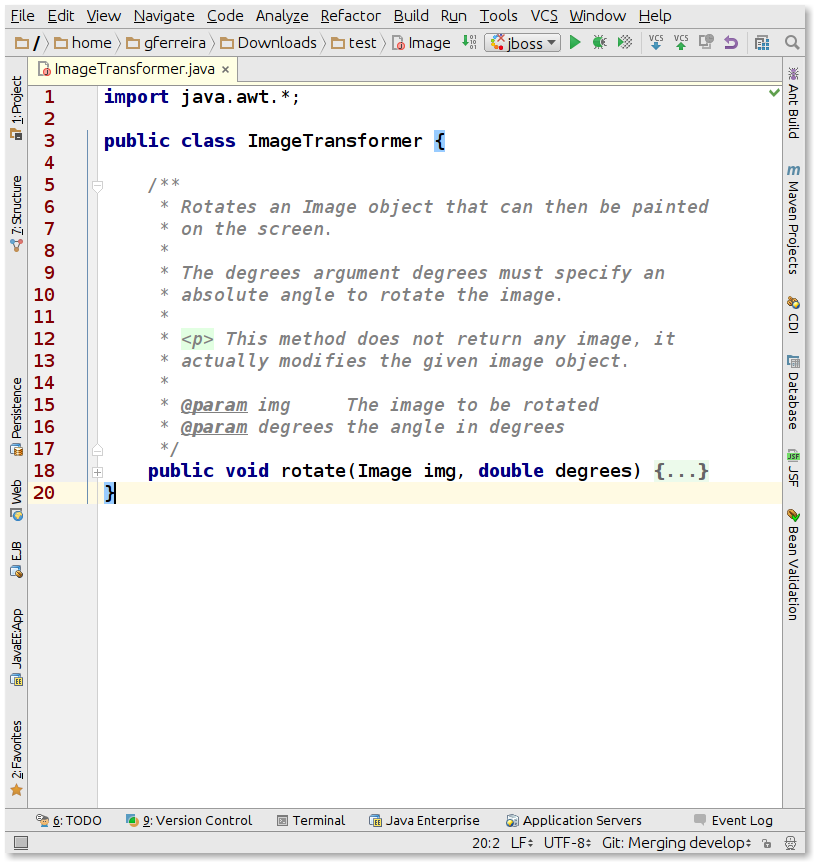
\includegraphics[width=.9\linewidth]{images/javadoc-code}
  \caption{A Javadoc annotation of a Java method}
  \label{fig:javadoc-code}
\end{subfigure}%
\begin{subfigure}{.5\textwidth}
  \centering
  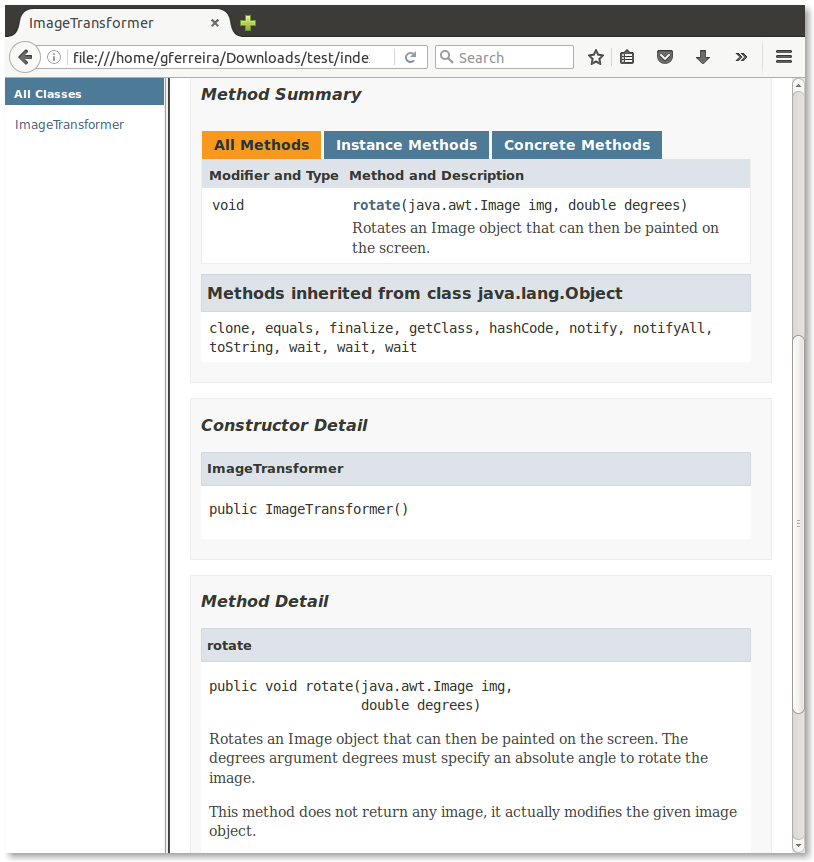
\includegraphics[width=.9\linewidth]{images/javadoc}
  \caption{Javadoc HTML auto-generated}
  \label{fig:javadocgen}
\end{subfigure}
\caption{Javadoc generation of a HTML page from a documented Java method. In the left is the source code commented with the opening tag \texttt{/**}, in the right is the generated documentation page.}
\label{fig:javadoc}
\end{figure}

Figure~\ref{fig:javadoc} shows an example of Javadoc, an industry standard tool which provides interesting functionalities for documenting Java classes. The HTML format keeps information together giving the convenience of being able to hyperlink related documentation. As a result, programmers can easily navigate through classes and their respective methods. Moreover, Javadoc provides a widely integration trough \glspl{ide} (e.g. Eclipse, IntelliJ, NetBeans, etc) so programmers can generate automatic Javadoc comments using those \glspl{ide}. However, this kind of tools is inadequate for another purpose.

For example, the documentation is essentially represented as rows of plain text. Despite supporting the HTML format, the generated pages only includes text and hyperlinks; media-rich resources are unsupportable. Moreover, the developer's attention is taken from code into a series of static pages which might contain little information and show less than the source code. Moreover, the automatic comments generated by some \glspl{ide}, are usually useless (e.g. a method called \texttt{getFoo()} would be automatically commented as ``This method gets a foo"). Finally, these tools are more focused on creating an industry standard, than properly documentations that effectively helps developers to comprehend the code and its architecture.

The representation of source code dramatically affects its comprehensibility and usability~\citep{baecker1986design}. The idea of enhancing program comprehension and usability by improving its representation using richer media resources is not new in the literature~\citep{marcus1982graphic,baecker1986design,baecker1983enhancing}. This research defines design principles for enhancing program visualization, showing the impact of those principles in the readability of the code. Based on these works, subsequent investigations and implementations have tried to keep those beliefs alive inside the academic context. For example Barista~\citep{ko2006barista} implements some of these principles  allowing media-rich annotation in the code editor (see Figure~\ref{fig:barista}), while Codelets~\citep{oney2012codelets} focus on supporting media-rich resources in code completion by enabling HTML icons visualization (see Figure~\ref{fig:codelet}) helping developer to write HTML pages 43\% faster than when using a standard Web browser\citep{oney2012codelets}.

\begin{figure}[h]
\centering
\begin{subfigure}{.5\textwidth}
  \centering
  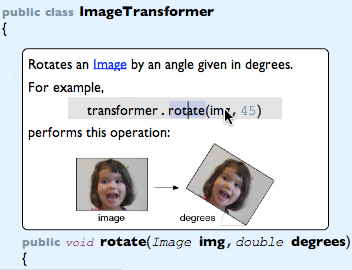
\includegraphics[width=.7\linewidth]{images/barista}
  \caption{A media-rich annotation in the Barista editor}
  \label{fig:barista}
\end{subfigure}%
\begin{subfigure}{.5\textwidth}
  \centering
  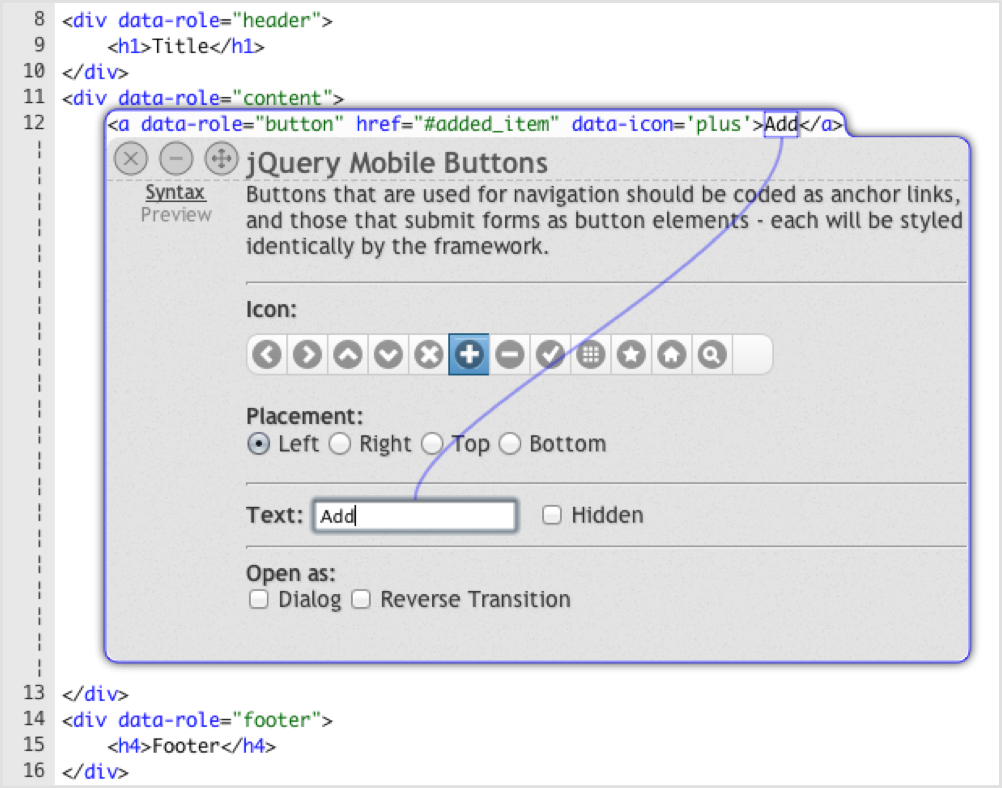
\includegraphics[width=.7\linewidth]{images/codelet}
  \caption{A Codelet inline helper}
  \label{fig:codelet}
\end{subfigure}
\caption{Example of media-rich annotations supported by code editors. On the left is Barista editor showing a Java method with richer annotations including images. On the right is the Codelets implementation showing the inline helper with icons defined for mobile buttons.}
\label{fig:richmedia}
\end{figure}

Barista~(Figure~\ref{fig:barista}), as a research project, is full of useful ideas for implementing interactive features in a code editor. Incremental parsing and a separation of \gls{ast} and view model of a source, is a useful concept. Moreover, it proposes tools such as media-rich annotation of methods (including hyperlink and diagrams inside the comments; allowing show/dismiss the comments by double clicking), readable pretty-printed view of formulas (enabling edit of these expressions by double clicking), and so on. As an implementation, however, the Barista source code (i.e. the used programming language Citrus~\citep{ko2005citrus}) is over ten years old and not maintained~\citep{contact:ko2006barista}. On the other hand, Codelets~(Figure~\ref{fig:codelet}) uses media-rich resources to present in a pop-up a variety of icons that develops can choose to create their web pages. However, it is more related to code completion technologies than support program documentation.

\subsection{Tools for documenting Generative Design programs}
\label{subsec:gdprograms}

Considering the \gls{gd} area, the lack of tools that accurately document a program, or automates the process of documentation, is still a problem. The absence of such mechanism discourages the process of documenting a program. Therefore, programs without documentation become difficult to understand, modify and eventually reuse. Consequently, this negatively affects the entire \gls{gd} community, once documentation plays a fundamental role in the development process. 

Unfortunately, the support for implementing the interactive tools presented above, and many other potentially useful tools, are weak or even inexistent in the majority of \gls{gd} systems. For example, in DesignScript~\citep{aish2012designscript}, Monkey, and many other textual environments, the source code is visually represented as rows of plain text, which makes difficult or even impossible the inclusion of rich-media elements (as shown, for instance, in Figure~\ref{fig:barista}). In the other hand, the visual programming languages, supported by environments such as Grasshopper and Dynamo, represent the source code visually with boxes and lines. However, to document these visual programs usually a box of plain text are provided, so that users can place it anywhere. As a result, the documentation can be spread throughout the program, making it difficult to access.

This problem aggravates by the increasing use of \gls{gd} methods to support the design and conception of real architectural projects. An architectural project, just like a software project, has a design phase where architects study the problem which they want to solve, analyze eventual constraints imposed by the client or external factors, and then define a draft of the solution. At the end of this process, several artifacts are produced, such as diagrams and handmade sketches (as those portrayed in Figure~\ref{fig:sketch-fig}). These sketches are commonly used among architects since early days of architecture~\citep{do2001thinking}, because they represent a compact medium to convey complex ideas. The information generated in the design phase may be sufficient to model the main components of the project, serving as a start point, and a basis, to the development process. 

Figure~\ref{fig:sketch-fig}, shows the importance of this phase in the architectural conception. In this example the architect started by drawing a series of sketches annotating them with dimensional and spatial parameters such as height ($h$), diameter ($d$), the normal vector ($\vec{N}$), and vertex points (e.g. $P_0, P_1, P_2, ...$) of each shape (see Figure~\ref{fig:sketch-fig}). These forms are treated as small components, that further can be combined to create new, different kinds of geometric objects. Understanding how these sketches are used in practice, is a crucial step before proposing any possible feature.

\begin{figure}[!h]
  \centering
  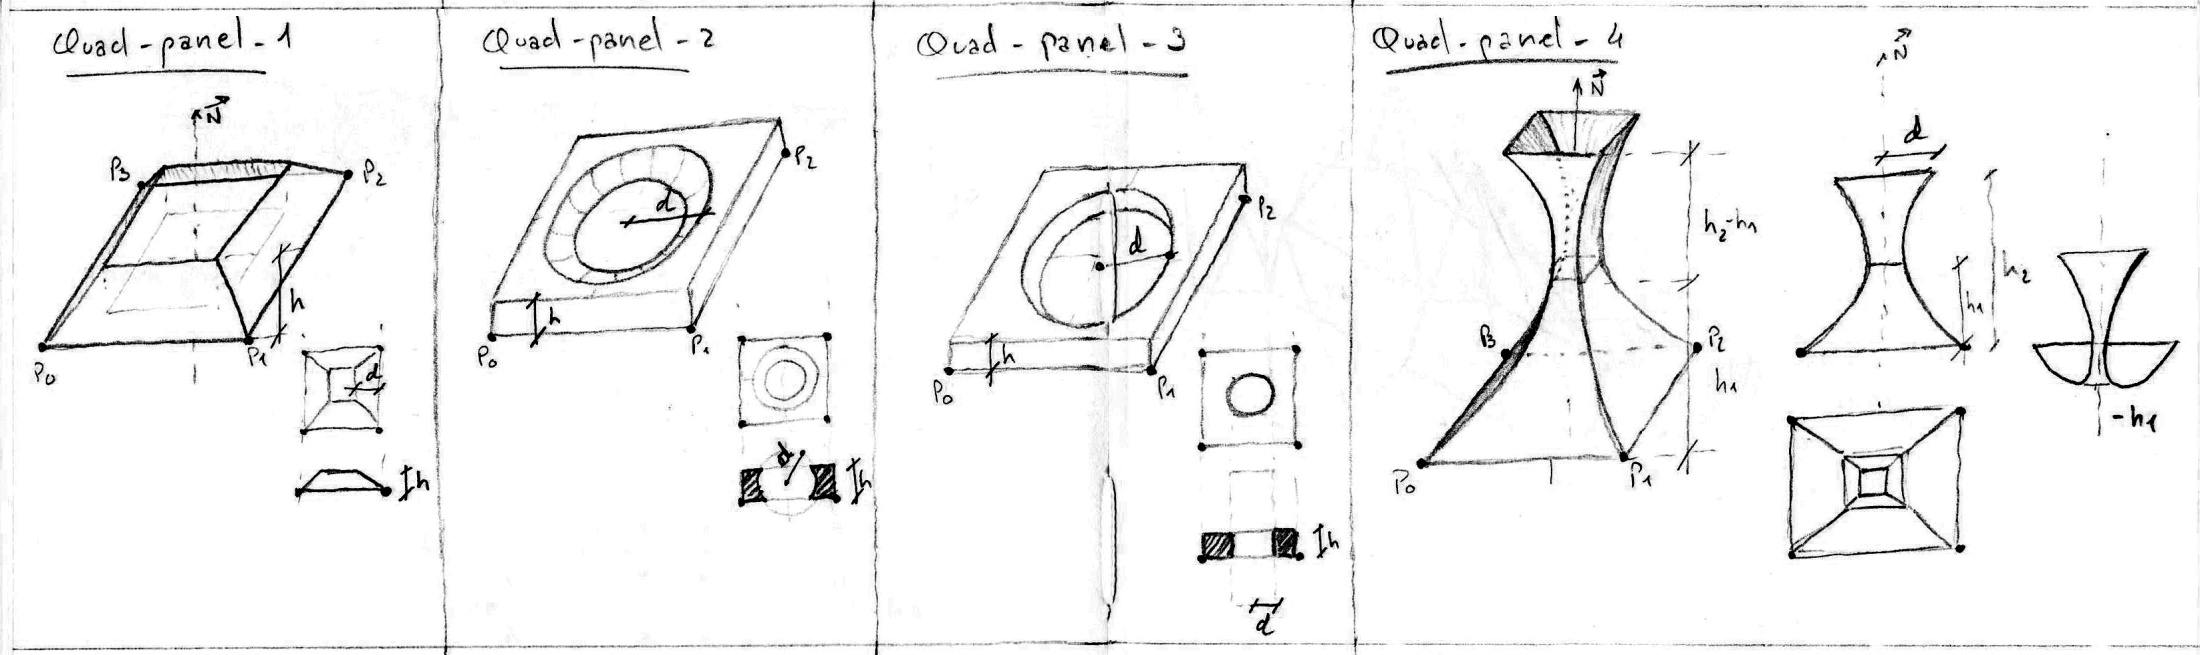
\includegraphics[width=1\textwidth]{images/real-sketch}
    \caption{Typical example of sketches made during architectural design phase.}
  \label{fig:sketch-fig}
\end{figure}

% \begin{figure}[h]
% \centering
% \begin{subfigure}{.6\textwidth}
%   \centering
%   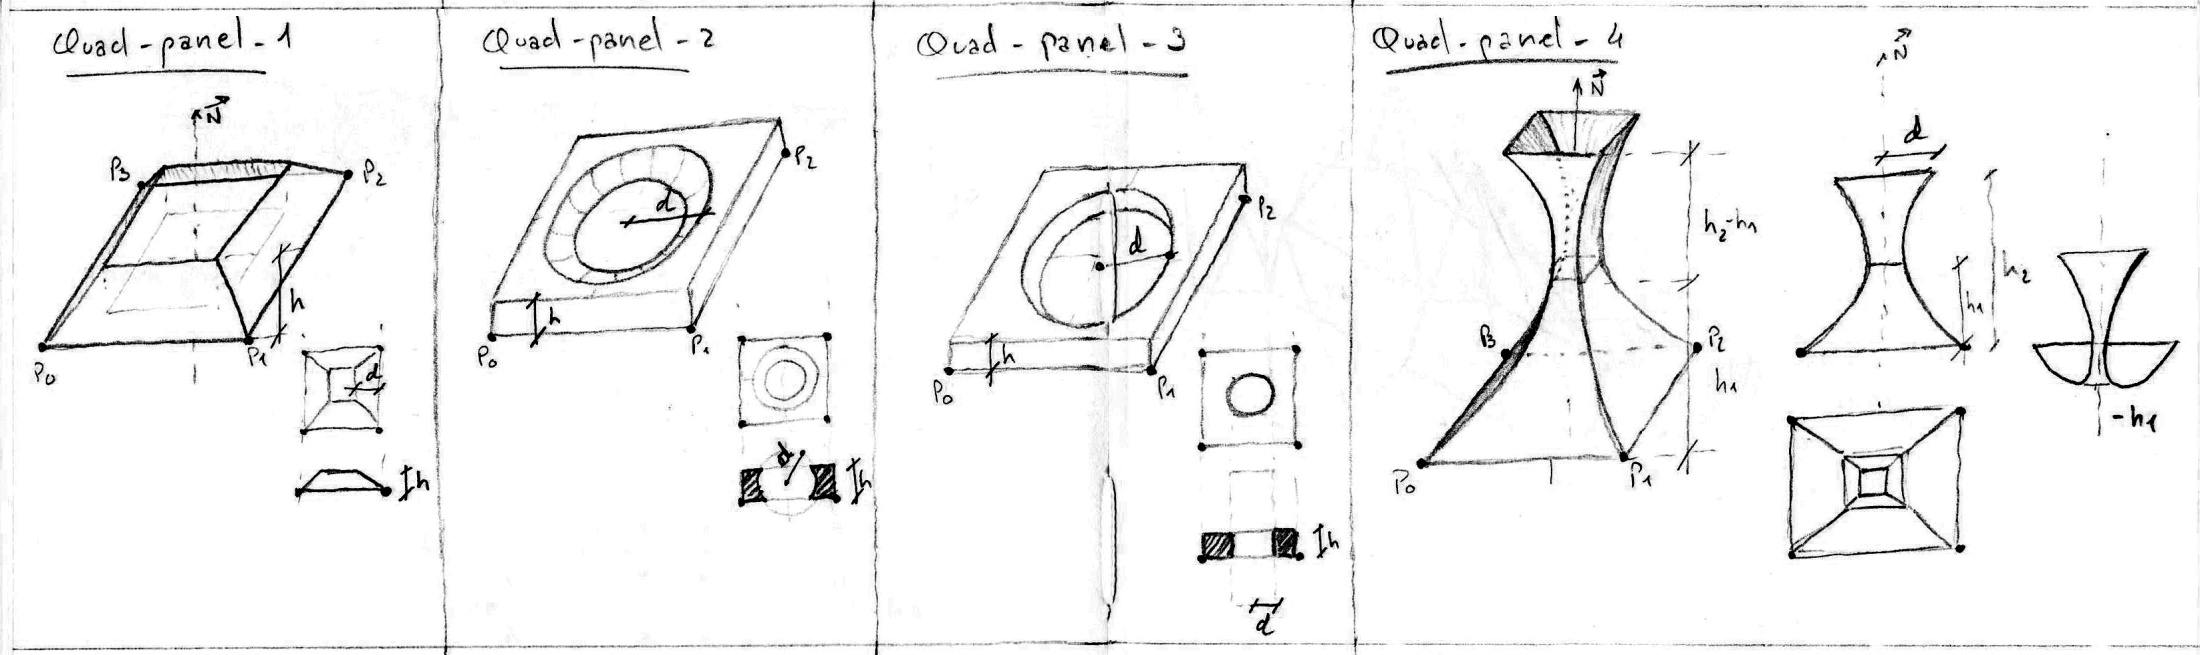
\includegraphics[width=.95\linewidth]{images/real-sketch}
%   \caption{Sketches made during architectural design phase}
%   \label{fig:sketch-fig}
% \end{subfigure}%
% \begin{subfigure}{.4\textwidth}
%   \centering
%   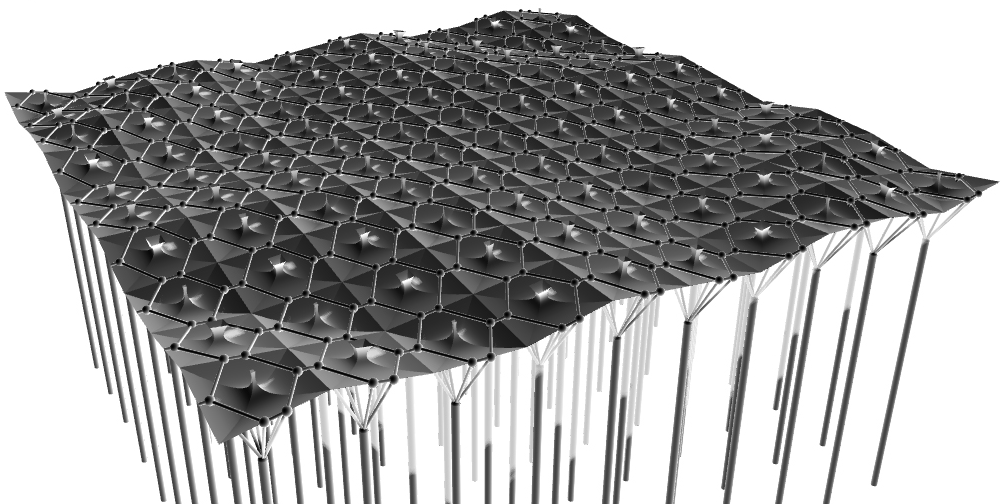
\includegraphics[width=1.0\linewidth]{images/real-sketch-result1}
%   \caption{An application of the objects modeled previously in an architectural model}
%   \label{fig:sketch-fig-result}
% \end{subfigure}
% \caption{Typical example showing the importance of design phase in the geometric model conception.}
% \label{fig:sketch-using}
% \end{figure}

By definition, a \gls{gd} method formally defines a description of an architectural model~\citep{mccormack2004generative}. In this way, while the code defines the geometric object textually, the sketch defines it visually. Consequently, the sketch is a rich source of information during the development of the program, and also after it, for documenting the program. Differently from the typical programs in software engineering, which are purely textual and may express concepts that are difficult or even impossible to represent graphically, the programs used in \gls{gd} have this capability of being able to represent its concepts through sketches or diagrams.

Moreover, illustrations and diagrams may help in the design conception because when the architect is doing them, he is thinking about the code to find a way to model a particular shape. At the end of writing the program, all architect's decisions and insightful design, applied to construct the final program, are encapsulated in these sketches. As a result, these sketches are also an essential artifact to comprehend the program, especially after its release. 

For example, consider Figure~\ref{fig:chairseat} that portrays a real example of a chair seat parametrically modeled. Even the less curious reader will wonder to know what each symbol of this image means. Some of them are more obvious than others, for instance, the angles and the differences between them. However, this diagram has its meaning embedded in problem context. It means that those symbols in the image are variables which were created purposely to solve the problem of setting up a different shape of seats by varying the variable values. So the sketch proposes a parametric model of the chair seat. Additionally, it contextualizes the meaning of each variable. Using this example, the architect can create a suitable \gls{gd} method that creates this chair seat. However, the \gls{gd} approach is not so straightforward as it seems to be. 

\begin{figure}[!htbp]
  \centering
  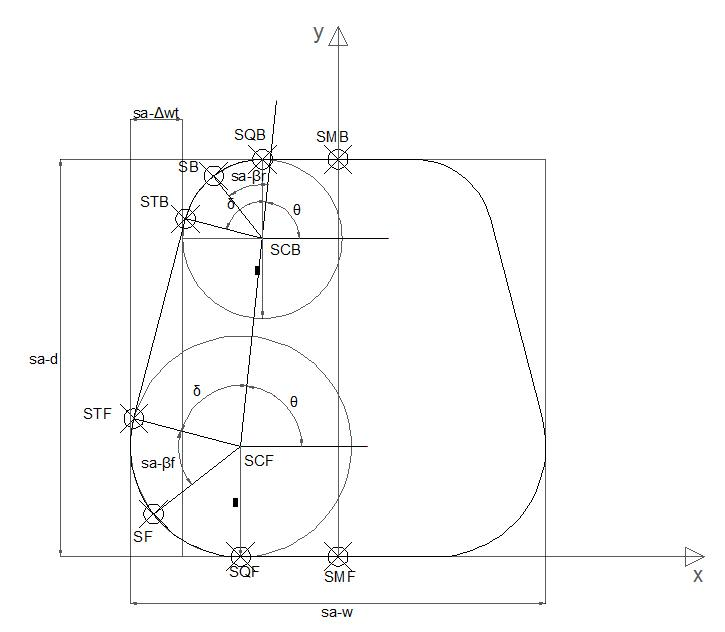
\includegraphics[width=0.8\textwidth]{images/seat}
    \caption{A real sketch of a chair seat. In this sketch, the seat is parametrized with some geometric variables. Some of them are intuitively noticeable, e.g. the angle symbols $\delta$, $\theta$, and $\beta$, but rest of them are not because they have its meaning embedded in the problem context.}
  \label{fig:chairseat}
\end{figure}

The problem with the \gls{gd} methods is that when a geometric model is translated into a programming language, the visual information that was available is lost. That is a serious problem for architects that do not have the same background of a software engineer, which means that visual models can be a preferred media for them, instead of interpreting symbols. 

% So, the sketches are an affluent source of information to guide the architect to comprehend the code. However when he look at the procedure that creates the model, he will see instead something like the following code, shown in Listing~\ref{lst:chairseat}. \\ [3mm]


For example, Listing~\ref{lst:chairseat} illustrates a function that models a chair seat with some of the parametric variables from Figure~\ref{fig:chairseat}. These variables are directly translated into function arguments. Therefore, when we look at this piece of code comparing it with the image, we understand the meaning of each variable, in the function context. Unfortunately, in most cases the sketches are not delivered with the program, even worst, the program is usually delivered without any documentation, or may have useless comments like that one in the example. Therefore, it negatively affects people who need to use this program, because without documentation they cannot understand the program well enough to use, or modify it, affecting the entire \gls{gd} community. \\

\begin{lstlisting}[
language=Python,
basicstyle=\ttm,
numbers=left,
stepnumber=1,
numbersep=5pt,                   
numberstyle=\scriptsize, 
caption={Python function that creates a chair seat given some of the parameters of Figure~\ref{fig:chairseat}},
label={lst:chairseat},
captionpos=b, 
otherkeywords={self},       % Add keywords here
keywordstyle=\ttb\color{deepblue},
emph={make_seat,__init__},       % Custom highlighting
emphstyle=\ttb\color{deepred},    % Custom highlighting style
stringstyle=\color{deepgreen},
numberstyle=\tiny\color{gray!110},
rulecolor=\color{gray!30},
frame=tb,                         % Any extra options here
showstringspaces=false,
backgroundcolor=\color{gray!5} 
]
def make_seat(smf, scf, scb, sa_d, sa_w, sa_deltawt, sa_betar, sa_betaf) :
   "this function creates a chair seat"
    ... # logic for creating a seat
    return seat;
\end{lstlisting}


\section{An approach for documenting Generative Design programs}

As discussed in the antecedent section, the lack of documentation in \gls{gd} programs negatively affects its users. In fact, this problem is beyond the \gls{gd} area; it also affects the field of software engineering. In this area, there were attempts to improve this issue by improving the quality of program documentation, most prominently, \textit{literate programming}~\citep{knuth1984literate}. This work proposed a programming paradigm that promoted the fact that programs are written for people first and foremost, and that documentation should be emphasized just as much as code. Unfortunately, these attempts did not reach the intended goals, mainly because writing good documentation takes a considerable amount of time and effort.

A more recent work~\citep{learnableProg} suggested that the programming environment should minimize this tough work, required to write documentation, by automatically providing the documentation that programmers need when they are reading the code. In this work, Victor outlines the following idea:

\blockquote{The environment is responsible for making meaning transparent. The environment must enable the reader to effortlessly read the program, to decode the code so that he can concentrate on genuine programming concepts~\citep{learnableProg}}

Figure~\ref{fig:victor-ex} shows a prototype, presented with this work, which demonstrates how the environment can improve the program readability. The code, on the left, is written in the Processing language~\citep{Reas2006}, it sets the environment color to green and creates two geometric objects, visible on the right, a circle and rectangle, using the Processing functions: \texttt{fill}, \texttt{ellipse}, and \texttt{rect}. This programming environment makes the meaning of each element of code transparent, providing labels on mouse-over. For example, when the reader points to the fourth parameter of function \texttt{rect}, he will know that it changes the height of the rectangle. Furthermore, he can also point to every element of this code to get its meaning, so before he makes any modification in the code, he will know what the code is doing.     

\begin{figure}[!h]
  \centering
  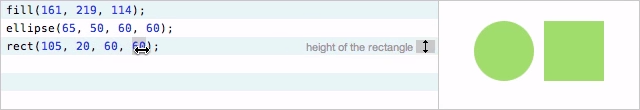
\includegraphics[width=.7\textwidth]{images/victor-example}
    \caption{A programming environment that helps in the program readability. On the left, is a sample of code, written in the Processing language, that creates a green circle and rectangle. On the right, is the result of this code. Each element of this program, including the functions and its arguments, are labeled, so when the user points the mouse over an item its label appears in the text editor.}
  \label{fig:victor-ex}
\end{figure}

Labeling the program elements on mouse-over indeed makes the program meaning more explicit, but this technique does not replace the need for proper documentation. The main problem with this approach is that these labeled functions already exist in Processing, so this feature is more intended to avoid unnecessary searches on the Processing User Manual than to provide a way to document the program. For any user-defined function this feature will be useless. Therefore, the developer must take a considerable amount of time and effort to create its documentation.

The reality in architecture is quite different from that in software engineering: \textit{it is part of the design process to produce documentation in the form of sketches}. This means that it is not necessary to write huge amounts of textual documentation to explain a \gls{gd} program. We only need to annotate the already existing sketches and combine them with the program, thus providing visual explanations of what the program is supposed to do.

\subsection{Sketch-program correlation tool}
\label{subsec:sketchtool}

Therefore, I propose a \textit{sketch-program correlation tool} that shows how sketches, made in an early phase of program design, can be combined with code to provide useful documentation for the developer. Figure~\ref{fig:sc-tool} illustrates a function, called \pythoninline{draw_arrow}, that draws an arrow giving the base point $P$, the direction $\alpha$, the height $\rho$, and the width $\beta$ and size $\sigma$ of the arrow tip. This information is all condensed in the sketch. So, the idea is to take advantage of this fact by pointing out what is the meaning of each function parameter, found in the code, in the context of the sketch (and vice versa). In this way, when the user has the mouse over a function parameter he immediately sees its illustration in the sketch, and the inverse is also valid: when he moves the mouse over a symbol in the image he immediately sees its meaning in the code.

\begin{figure}[!htbp]
  \centering
  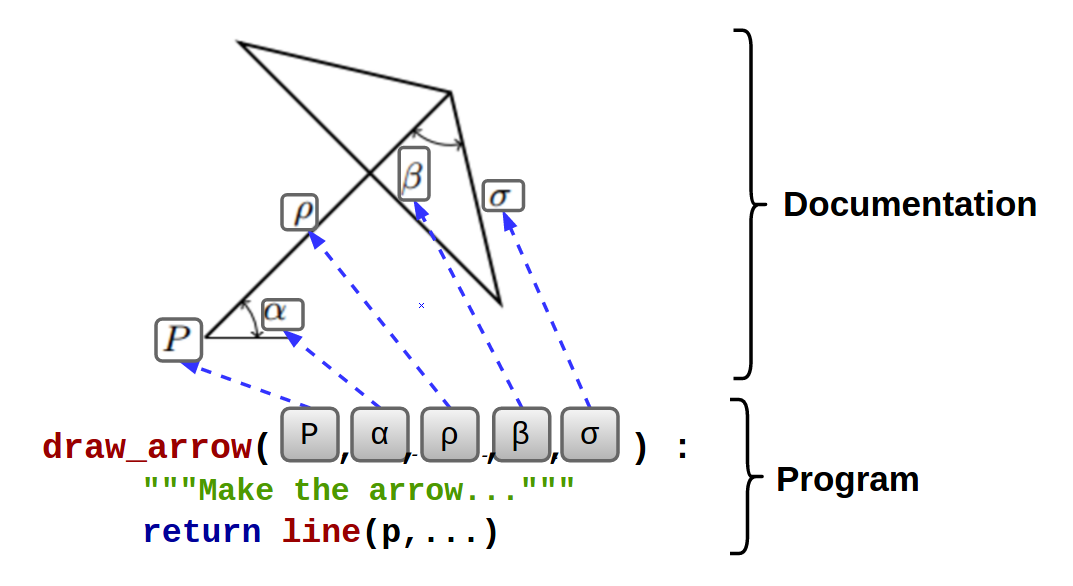
\includegraphics[width=0.6\textwidth]{images/proposed-sc-tool}
    \caption{\textit{Sketch-program correlation tool} showing how to combine fragments of the program with sketches.In this example, all the function parameters are linked to a  symbol in the sketch that illustrates its meaning.}
  \label{fig:sc-tool}
\end{figure}

As research, this tool presents a useful idea, as an implementation, however, this mechanism imposes hard challenges. For example, one of the first challenges is how to include images in the code editor. The majority of source code editors, currently used for textual programs, do not support this feature. We are not aware of any other source code editors, widely used, that provides such capability, except DrRacket~\citep{findler2002drscheme} that implements an enhanced editing mode with support for images and other media-rich elements.

\subsection{Dealing with images resources}

An inherent concern for supporting pictures in the code editor is how to store them. The strategy used by DrRacket~\citep{findler2002drscheme} is to serialize the image and save it in ASCII-encoded binary format. The problem with this approach is that, once the developer inserts an image in his code and keeps it, he will be unable to change its code again using a different text editor. So, this method does not provide any backwards-compatibility with other text editors potentially useful to write programs. As a result, it makes it difficult, or even impossible, to have portability of programs written in this programming environment with the different text editors widely used.

I suggest a different approach to this problem that assures backwards-compatibility among source code editors. In this way, the image is inserted inside a tag delimiter enclosed by a source code comment. For example, Figure~\ref{fig:inline-img1} shows a function, written in Python using a code editor that support images. This program has a  multiline source code comment, spanning multiple lines of text mixed with the image (starting and ending with the delimiter \texttt{'''}). Inside this comment is a tag, in XML, that specifies the information associated with the image, such as its location, its parameters, and also the place of each parameter in the picture. The programming environment loads this information upon a picture insertion event. However, users can edit this fields after the image is loaded.

\begin{figure}[h]
\centering
\begin{minipage}[b]{0.49\textwidth}
  \centering
  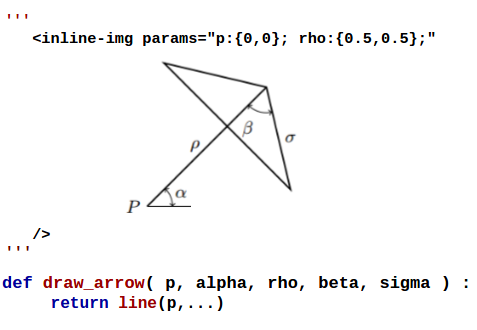
\includegraphics[width=1\linewidth]{images/inline-img1}
  \captionof{figure}{Opening the source code in an editor that supports the \texttt{inline-img} annotation.}
  \label{fig:inline-img1}
\end{minipage}%
~
~
\begin{minipage}[b]{0.49\textwidth}
  \centering
  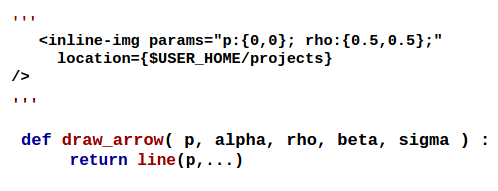
\includegraphics[width=1\linewidth]{images/inline-img2}
  \captionof{figure}{Opening the source code in an editor that does not support the \texttt{inline-img} annotation.}
  \label{fig:inline-img2}
\end{minipage}
\end{figure}

The advantage of this mechanism is that when users open this code in a text editor that does not support images, they can access the source code entirely, as shown in Figure~\ref{fig:inline-img2}. However, the images are not displayed. Instead, the source code comment shows the image path and associated information.  On the other hand, the disadvantage of this method is that pictures have to be bundled with the text file. Otherwise, the text editor will not find them, consequently, not displaying.

Other systems, to avoid this incompatibility problem,  convert the code, which includes media-rich elements, into a standard format. For example, Barista~\citep{ko2006barista} saves the code in XML. However, the presented approach goes further, because it does not impose any language specific requirement, the code is stored as it is (ordinary plain text). So it is up to the code editor to implement suitable methods to show the images.

\subsection{Automatically binding code with images}

Once we can insert images in the text editor, the next step is somehow associate these images with code. Figure~\ref{fig:sc-tool} shows a possible approach, where the function parameters point to the symbols in the picture. Note that; these symbols can be words rather than a single character. Thus, an interesting feature would automatically recognize these symbols, getting their optical character and respective position. Therefore, having this information makes it possible to match the parameters found in the code, with the symbols found in the image.

Recognizing text characters on images is an old problem. The very first attempts can be found back in 1870~\citep{eikvil1993optical} with the retina scanner which was an image transmission system using a mosaic of photocells. From then, consecutive attempts were made to improve this method especially by sophisticating the retina scanner and creating machines that became commercially available in the 1950's. Posteriorly, HP as a possible software and hardware add-on for HP's line of flatbed scanners, proposed a novel open-source project: Tesseract~\citep{smith2007overview} \gls{ocr} which aims to implement the scanner reader entirely in software. Thereafter, this project was sponsored by Google and nowadays is one of the most accurate \gls{ocr} engines on the market, widely used in several web applications.

Clearly, the subject of character recognition is extensive, and its details are beyond the scope of this dissertation. However, my solution for automatically recognizing text in images is based on an \gls{ocr} engine, namely Tesseract~\citep{smith2007overview}, that accepts an image as input and returns a file with the known characters and their respective coordinates as output. However, Tesseract is a local C++ application that needs to be installed on the user's computer or included as an external library, which may affect the portability of the application and its use.

To overcome this limitation, I propose the use of \gls{ocr} Web Services, such as OnlineOCR\footnote{\texttt{http://www.onlineocr.net/}}, or FreeOCR\footnote{\texttt{http://www.free-ocr.com/}}, as these engines provide the same functionality as Tesseract and, in fact, most of them are build on top of it. Moreover, as web services, these systems provide a straightforward integration with external applications, once they use standard protocols, such as SOAP, or REST. In Figure~\ref{fig:sc-tool-arch}, I suggest an architecture for integrating the \gls{ocr} engine as a module of this tool. This architecture describes a data flow view, starting when users insert an image in the editor, until the end of the process when the editor saves the image. Thus, the components of this architecture are described as follows:

\begin{itemize}
\item \textit{Code Editor.} It is the main \gls{ui} for the programmer where he will write code and insert images. So, this component is the initial filter of the pipe. Consequently, it starts the logic sequence flow for processing the image.

\item \textit{Image Filter.} This component has two principal activities: first get the image inserted into the text editor, and second send the image to the \gls{ocr} engine through REST invocation. (Note: it assumes that the web service provides a suitable service for this invocation, which is naturally expectable among the \gls{ocr} Web Services studied.)

\item \textit{OCR Engine.} It is the fundamental piece of this architecture, from where the image will be processed and transformed into optical characters. This component is the most critical of this architecture because the correct operation of this tool depends on how well this engine will operate.

\item \textit{Meta-data Collector.} This component is intended to receive the information processed by the \gls{ocr} engine, and then stores it. This information contains the recognized optical characters and, additionally, the coordinates from where the \gls{ocr} picked each symbol. 
\end{itemize}

\begin{figure}[!h]
%\vspace{-5pt}
  \centering
  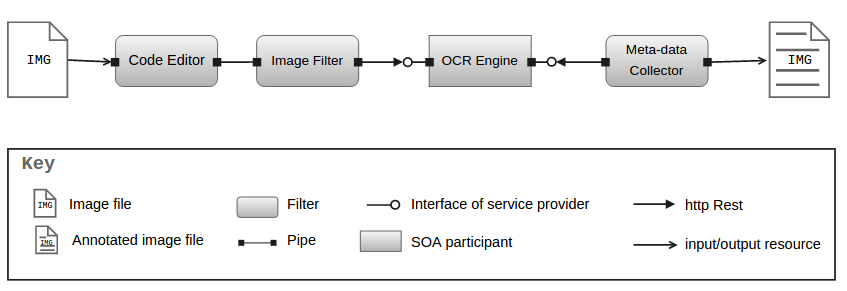
\includegraphics[width=.7\textwidth]{images/sc-tool-architecture}
    %\vspace{-15pt}
    \caption{The suggested architecture for integrating the \gls{ocr} Engine. This architecture presents a data flow view combining two styles: pipe-and-filter style and client-server style.}
    %\vspace{-5pt}  
  \label{fig:sc-tool-arch}
\end{figure}

The presented architecture left several unclosed questions, for example, a clear issue is where the \textit{Meta-data Collector} will store the information received. This decision is hard to make now because it is intrinsically related to the way which the programming environment stores its rich-media elements. As discussed earlier, there are several approaches to deal with it, such as serialize the items in a binary format, use standard formats such as XML, and, our own approach: use common source code comments to wrap the media-rich information. The strategy used for storing meta-data with the image may vary depending on the output format chosen. What I propose is to use the last option, due to the backward-compatibility among different text editors.

\subsection{Designing a fallback mechanism}

Unfortunately, the \gls{ocr} engine uses a pattern recognition technique which is susceptible to errors. To overcome this problem, I propose a \textit{fallback mechanism} that delegates the task of recognizing symbols to the programmer. Thus, the programmer can directly intervene in the image recognition process helping the \gls{ocr} upon mistakes. Moreover, the user input can be a rich source of information for the \gls{ocr} engine because this data can be used as a corpus of training, therefore improving its recognition capabilities. After processing the image and obtaining the contained annotations, the next step is to present this information meaningfully.

\subsection{Presenting binding associations}

At this point, we have the code and the annotations extracted from the image, then the goal is matching them. I propose two alternatives to overcome this problem, as follows:

\begin{enumerate}
\item \textit{Implement a programming environment from scratch.} This option allows a high level of customization because the environment will be built based on this requirement. Thus, adequate technologies can be chosen purposely to deal with images in code and support the binding between code and image, as shown in Figure~\ref{fig:sc-tool}. Moreover, this tool can be language-independent, to correctly operate it only requires access to the image meta-data and the syntactic structure of the program, generated in compiling phase, i.e. the \gls{ast}. This approach can also minimize the effort to add additional features because different tools share the same core implementation. Despite the clear advantages, it requires a huge effort to implement such environment and, of course, a risk that this environment will be considered useless by the target users. For example, Barista~\citep{ko2006barista} takes this approach, providing an environment for Java programmers. However, it is very unlikely that a Java programmer will use this tool in his daily tasks.

\item \textit{Extending an existing programming environment.} This is a more straightforward approach, based on the fact that most programming environments nowadays provide some support for add-on features. In this way, programmers can create new features without changing the programming environment itself by implementing a common \gls{api}. The main advantage of this approach is that we can use resources generated by other tools without having to apply them. For example, the \gls{ast} which is a rich resource generated during the compiling phase, is usually provided through \gls{api} methods. Alternatively, the programming language can be used to achieve this goal; some programming languages allow the definition of new grammar rules. As a result, a new grammar rule can be created to consider images as part of the programming language grammar. However, this approach is extremely dependent on the language/environment support for add-ons and, therefore, of the \gls{api} provided to extend the system.
\end{enumerate}

\subsection{Strategies to improve the usability in the source code editor}

An important issue that affects the entire system is related to the usability of the programming environment. Adding images mixed with code is something that can impair the usability of the programming environment because images can occupy a considerable part of the text editor making the program readability more difficult. Moreover, when programmers are coding, they are focusing on that task and the images might be a distraction. This is a problem that does not have a straight solution. However, I propose some strategies to handle the problem:

\begin{itemize}
\item Treat rich-media resources, including images, as text. It means that programmers should be able to work with these resources just like they do with text so that it can be cut and paste, it can be deleted, it can be moved by dragging and drop, and it can also be indented.

\item Support text caret navigation as in a text editor. Evidence from a study of programmers' low-level text editing strategies~\citep{ko2005design} suggests that programmers rely heavily on the keyboard for code navigation. Therefore, adding rich-media resources in the source code can interfere with the caret navigation. However, treating images as text will not affect the caret navigation.

\item Show or dismiss the rich-media resources by double clicking. The purpose of this facility is to avoid distractions, so when the programmer is coding he clicks over the image, to dismiss it and focus on the code editing.

\item Add images by dragging and drop and support inline edition. It is important for the users that adding images, or other resources, be as simple as writing code. Mechanisms such as drag and drop, edit the picture directly in the text editor, among others facilities, should be considered. The fewer iterations are needed to select an image, the better it will be the user experience.
\end{itemize}

\section{Immediate feedback}

Programming requires developers to maintain many different kinds of ‘mental models'~\citep{brooks1977towards,robins2003learning}, which represents how they comprehend the code. Therefore, after writing a single line of code, intellectual work must be done in the developer's mind. During this phase, the developer is formulating several theories about the program. However, he can only test these ideas when he found evidence in code. Which means that, he needs to edit the program, compile the code and execute it to test if his theories were right or not.

There were several attempts to facilitate this process, trying to make programming in a more concrete task. For example, the invention of debugger tools was precisely to enable programmers to see the state of their programs, its structures, and how the flow of information passes through it upon execution. With successive improvements of these tools, modern systems, such as LightTable~\citep{lighttable}, have been trying to anticipate as much as possible the result of a program change. This environment reduces the delay between an edition in the source code and the visualization of its effect. Although this is a simple concept in practice, it becomes popular in the academic community and even beyond it in the industry context. For example, JRebel\footnote{\texttt{https://zeroturnaround.com/software/jrebel/}} is a popular tool that allows developers to visualize changes in a web application without stopping the application server. Visualizing changes allow programmers to test their mental models, therefore improving their comprehension about the program.

The smaller the delay between making the changes and visualizing their effects, the better. \textit{Immediate feedback} is, thus, when there is no perceived delay between the change and the effect. Therefore, immediate feedback accelerates the process of program experimentation so programmers can test their mental models faster, enhancing their program comprehension.

\subsection{Immediate feedback in Generative Design}

A good practice in Architecture, however, is the use of sketches to convey ideas~\citep{do2001thinking}. Sketches are, in fact, a suitable media to experiment, and test new ideas quickly, which is a fundamental requirement for creating novel designs. However, \gls{gd} methods drastically change this reality: instead of interacting directly with the model, as traditionally in Architecture, the architect interacts with a model's intermediate, i.e. the program that specifies it. Thus, any change in the model must be performed first in the code and then, only after the execution of the program, the architect will be able to see the impact of his change in the model. This process delays the visualization of the model, negatively affecting the design process.

To overcome this limitation, notable efforts have been made in the \gls{gd} area. For example, visual programming languages, such as Grasshopper~(see Section~\ref{subsec:grasshopper}) and Dynamo~(see Section~\ref{subsed:dynamo}), provide immediate feedback. Therefore, as the user interacts with the language components, by adding and connecting them, the effect of this interaction is immediately available in the \gls{cad} model. However, in these visual programming languages, as programs become large and complex it requires more time to understand, maintain, and adapt to new requirements~\citep{leitao2011programming}. Moreover, the delay between changes and visualization increases, making immediate feedback impossible. On the other hand, programming environments for textual languages do not support immediate feedback at all.

\subsection{Immediate feedback tool}

To change this reality, I propose an immediate feedback tool aimed for textual programming languages. The goal of this tool is to substantially reduce the time between a change in the code, and its effect in the program execution. Therefore, architects will be able to improve their programs and see the impact of that change in the geometric model, allowing \textit{program experimentation} and, eventually, improving \textit{program comprehension}. Moreover, this tool provides a foundation for other features, which can be implemented on top of it. 

For example, a useful tool that promotes program experimentation is the use of widgets to change the program input. Moreover, using immediate feedback feature is possible to improve the \textit{autocomplete} mechanism. In this way, and different from the traditional \textit{autocomplete} tool that shows a list of options suitable for a particular expression, this mechanism can do more, so when architects select an expression in the list of choices, the selected expression is sent to the immediate feedback tool and its result becomes immediately available.


\subsection{The activities of program experimentation}

However, to improve program experimentation process we need first to find the activities of this process, especially the most time-consuming. For example, using the parametric model shown in Figure~\ref{fig:chairseat}, is possible to generate a set of chair seats. To this end, the architect, using the implementation of this model, can proceed as shown in Figure~\ref{fig:run-activity}, where these activities are described as follows:

\begin{itemize}
\item Find places to change in the source code. The time spent to perform this task may vary substantially, depending on the complexity of the program, and the architect's knowledge about the program. Unfortunately, these factors are not directly related to this tool; it is more associated to the tool presented in Section~\ref{subsec:sketchtool}.

\item Edit the source code, choosing suitable program inputs to perform the desired action. Considerable time is spent in this activity because architects usually need to predict the range of values that makes sense for each program parameter. Fortunately, this operation can be improved by this tool, saving any wasted time spent on it.

\item Run the program. Depending on the programming environment this step can be a simple button click, up to execute a command to compile, and run the program. This step can be optimized using appropriate techniques, such as reusing the previous computation.

\item Visualize the change in the model and check if it was sufficient to generate the desired model, otherwise, repeat the process. As a result, this is one of the most time-consuming activity, because it relies on the \gls{cad} tool to generate the model. As discussed in the previous sections, \gls{cad} tools are not designed to process the huge amount of information produced by \gls{gd} methods. Therefore, alternative visualization devices must be considered to optimize this activity.   
\end{itemize}

\begin{figure}[!htbp]
  \centering
  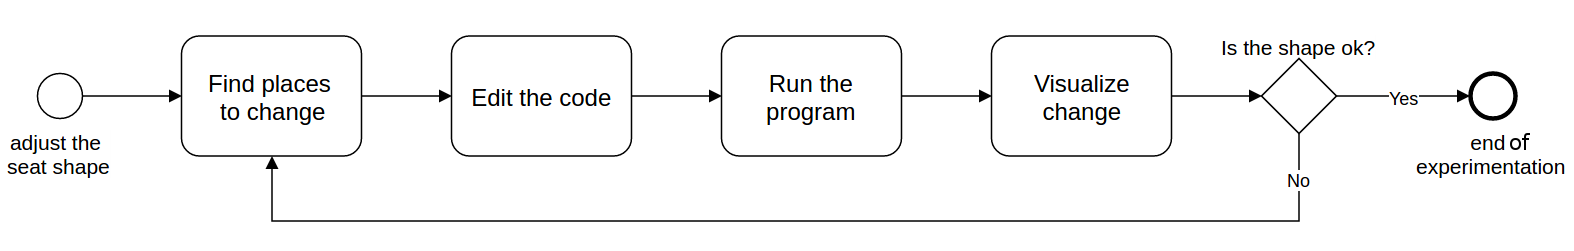
\includegraphics[width=1\textwidth]{images/run-activity}
    \caption{Activity diagram for generating a set of seat shapes.}
  \label{fig:run-activity}
\end{figure}

\subsection{Improving program execution}

Base on these activities, a first approach would be optimizing the program execution. Some programming systems, such as Impromptu~\citep{sorensen2005impromptu}, and Fluxus \citep{griffiths2007fluxus}, attempt to address this with \textit{"live coding" environment}, where the program output updates immediately as the code changes. These systems use a standard technique to provide this feature: a language interpreter that given an expression directly evaluates it. Curiously, both of them use the Scheme interpreter (a Racket~\citep{findler2002drscheme} ascendant) due to its enhanced capability for evaluating expressions, and ease integration. For example, the Scheme runtime can be integrated with other programming languages like C, and C++, the interpreter already provides a sandbox mechanism, only executing code syntactically correct, thus avoiding compilation errors. However, in these programming systems change in the code causes the interpreter to evaluate the entire program again.

An apparent gain in performance is related to the utilization of the previous computation that was unchanged after a code edit. For example, consider the sample of code, shown in Listing~\ref{lst:offset}, that creates a chair given a point, the chair height and width, and the seat dimensions.

The function \pythoninline{create_chair_obj}, at line 5, does the major part of the computation, creating the chair object, and the function \pythoninline{move_to}, at line 6, only translates the model to the given point. If the architect moves the chair position (e.g. change it to $\{ x\!=\!1,y\!=\!1,z\!=\!1 \}$) is unnecessary to create another chair, once this change does not affect the chair shape. In this way, the operation will be a simple translation. However, this solution will not work in some cases. For example, the global variable \pythoninline{offset} is a constant for the program. Therefore, a standard compiler optimization known as constant folding will replace every occurrence of that variable by its value. The resulting program is shown in Listing~\ref{lst:offset-change}.


\begin{lstlisting}[
language=Python,
basicstyle=\ttm,
numbers=left,
stepnumber=1,
numbersep=5pt,                   
numberstyle=\scriptsize, 
caption={Python program that creates a chair.},
label={lst:offset},
captionpos=b, 
otherkeywords={self},       % Add keywords here
keywordstyle=\ttb\color{deepblue},
emph={make_chair,__init__},       % Custom highlighting
emphstyle=\ttb\color{deepred},    % Custom highlighting style
stringstyle=\color{deepgreen},
numberstyle=\tiny\color{gray!110},
rulecolor=\color{gray!30},
frame=tb,                         % Any extra options here
showstringspaces=false,
backgroundcolor=\color{gray!5} 
]
offset = 50
def make_chair(p_center, ca_h, ca_w, sa_d, sa_w) :
   real_p = xyz(p_center.x/offset, p_center.y/offset, p_center.z/offset)
   # some complex computation
   chair = create_chair_obj(ca_d, ca_w, sa_d, sa_w)
   return move_to(real_p, chair)
# creates a chair in origin
make_chair(xyz(0, 0, 0), 20, 20, 30, 30)
\end{lstlisting}

\begin{lstlisting}[
language=Python,
basicstyle=\ttm,
numbers=left,
stepnumber=1,
numbersep=5pt,                   
numberstyle=\scriptsize, 
caption={Python program that creates a chair, after constant folding.},
label={lst:offset-change},
captionpos=b, 
otherkeywords={self},       % Add keywords here
keywordstyle=\ttb\color{deepblue},
emph={make_chair,__init__},       % Custom highlighting
emphstyle=\ttb\color{deepred},    % Custom highlighting style
stringstyle=\color{deepgreen},
numberstyle=\tiny\color{gray!110},
rulecolor=\color{gray!30},
frame=tb,                         % Any extra options here
showstringspaces=false,
backgroundcolor=\color{gray!5} 
]
offset = 100
def make_chair(p_center, ca_h, ca_w, sa_d, sa_w) :
   real_p = xyz(p_center.x/50, p_center.y/50, p_center.z/50)
   # some complex computation
   chair = create_chair_obj(ca_d, ca_w, sa_d, sa_w)
   return move_to(real_p, chair)
# create a chair in (1,1,1)
make_chair(xyz(1, 1, 1), 20, 20, 30, 30)
\end{lstlisting}

The problem happens if the architect decides to change the value of \pythoninline{offset} (at line 1). This alteration will have no effect on the program output, because the \pythoninline{make_chair} is reusing a previous computation where the \pythoninline{offset} was defined as 50, so the code must be compiled again to reflect this change. Consequently, the technique of reusing the previous computation will be in vain.

However, there are other approaches to this technique. For example, the Design Script~\citep{aish2012designscript} language implements a data flow paradigm, creating a dependency graph between variables. In this case, \pythoninline{offset} will be linked to its usage (the three parameters of Listing~\ref{lst:offset-change}, at line 3). So, changing its value, will cause a recalculation of these parameters.  On the other hand, YinYang~\citep{mcdirmid2013usable} will compile just the changed branch in the \gls{ast}. However, these languages were tailored specifically for this purpose and are outside the scope of this thesis.

\subsection{Program experimentation in Generative Design}

A relevant issue associated with textual programming environments in \gls{gd} is the lack of tools that facilitate program experimentation. Each time the architect wants to change a geometric model, he needs to edit the code blindly, guessing an appropriate input for that parameter. Clearly, this is an ineffective way to test the program, besides of being a laborious process for experimentally generating new models,  discouraging the creative work.

Visual programming languages, such as Grasshopper and Dynamo, understand this as a severe limitation for the architectural work. They provide some mechanisms such as interactive widgets, e.g. sliders, which facilitate the process of program experimentation. For example, in Grasshopper users can add a slider in component inputs, as shown in Figure~\ref{fig:grass-con}. Therefore, the slider is defined in a range of values, and each time the user drags the slider the program is executed with that input.

\begin{figure}[h]
  \centering
  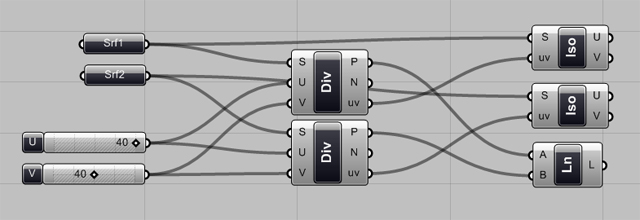
\includegraphics[width=0.65\textwidth]{images/grass-connections}
    \caption{A Grasshopper program. On the left, is the program inputs connected by sliders. On the right, are the program components.}
  \label{fig:grass-con}
\end{figure}

A similar technique, is used in live-code environments like Fluxus~\citep{griffiths2007fluxus} and Impromptu~\citep{sorensen2005impromptu}. Although these programming systems are associated with textual programming languages, they provide sliders to allow performers to change their program inputs. In a live code presentation, performs use their programs to impress the audience. In this situation,  sliders are crucial to change the program inputs. Therefore, in these systems sliders are an indispensable feature, so they are part of the programming environment. However, other textual programming systems, such as DrRacket, provides a \gls{gui} library for input widgets, such as a slider. Therefore, sliders are create outside the programming environment, which means that users define the slider in their source code, and upon program execution, the slider is displayed in an \gls{ui} frame. 

To create a new slider, in DrRacket, users must specify a label, a max-range, a min-range, and a function callback. The slider callback can be associated with an existing function,and each of its parameters can be linked to a slider. Then when the slider is moved the callback executes the function with the selected values. For example, Figure~\ref{fig:slider-ui} shows the slider associated with the function illustrated in Figure~\ref{fig:sc-tool}. 

\begin{figure}[h]
  \centering
  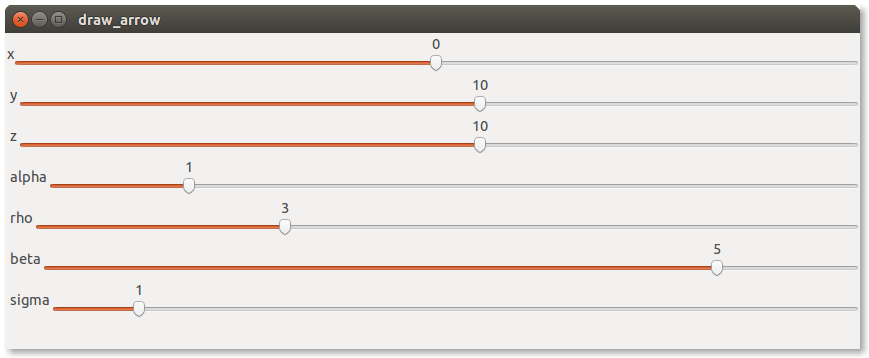
\includegraphics[width=0.6\textwidth]{images/slider-sample}
    \caption{A slider user interface for the \texttt{draw\_arrow} function.}
  \label{fig:slider-ui}
\end{figure}

In fact, the \gls{ui} shown in Figure~\ref{fig:slider-ui} allows the function \pythoninline{draw_arrow} be executed interactively. However, this \gls{ui} only executes the \pythoninline{draw_arrow} function, because its callback is associated to this function. So, for any different function, the user must create a new slider, defining all the required parameters again. Moreover, as numerous are the parameters of the function, as greater will be the \gls{ui}. Therefore, it can reach a point that can disturb the developers, and, even worst, it hides the surrounding context from where the function is called.

\subsection{Inline sliders mechanism}

To overcome these limitations, I propose a slider mechanism that is integrated in the programming environment. So, it facilitates the change of each program literal individually. Instead of showing the \gls{ui} with the function parameters at once (as shown in Figure~\ref{fig:slider-ui}), this mechanism allows each function parameter to be changed individually, creating a unique slider on top of that parameter. As a result, programmers can interactively modify the program input without losing the surrounding context of the program. Moreover, this mechanism is independent of the program execution, which means that dragging the slider will only make changes in the code. Obviously, to have an immediate effect on the program execution, the program should be executed at each slider change.

\subsection{An inherent problem}

Unfortunately, immediate feedback will not scale with the increasing complexity of \gls{gd} programs. When the programmer drags the slider, he is expecting to see how that alteration looks like in the model. Likewise, when we are writing in a text editor, we are hoping to see how the words appear in the text editor. Otherwise, we will probably think that something is going wrong. Show the program hidden states is an important heuristic, especially in a context where users are dependent on the program result. However, implement this heuristic in the current \gls{gd} environments would be a hard challenge.

Grasshopper is a concrete example of \gls{gd} system that has been facing this problem insistently. The initial approach was execute the program at each change. When the program becomes complex, its execution time get bigger and bigger, reaching a point where programmers become afraid to touch in the sliders to avoid freezing. To overcome this problem, a second approach was to restrict the slider input to only accept textual inputs. As a result, this method was highly criticized, because it was against the principles of visual programming languages. Thus, a new strategy was proposed: deactivate slider dragging effect and only reproduce the final dropped value. This strategy had a better performance, but it limits the program experimentation to individual points in the range of the slider. Obviously, this is not exactly a solution and will not solve the problem, only delays its onset.

Fortunately, there is a straight solution for this problem, as discussed above, which is sidestepping the most functionalities of \gls{cad} tools, using an alternative visualization device. For the purpose of this tool, I propose to use an alternative render device working as a kind of \textit{playground} where users can create samples, and find out the right parameters to build their models. Moreover, sliders can be used to create these models interactively.

\subsection{Adaptive sliders}

However, sliders must have helpful values that make sense for that program input. For example in Figure~\ref{fig:slider-ui}, the parameters showed have a distinct range of values, i.e. $\{x,y,z,\sigma,\rho\} \in \mathds{R}$, $\alpha \in [0, 2 \pi]$, and $\beta \in [0, \pi/2 ]$. The problem is how to predict an accurate range of values for a function parameter. In principle, the program variables declared as integer have their domain in $\mathds{Z}$, so the challenge is to restrict this domain to something that makes sense for that particular invocation. There are several strategies used in practice, for instance LightTalbe~\citep{lighttable} shows a drop down list where the first value is a minor value (i.e. $x \in \mathds{R}^- : x \rightarrow - \infty$) and the last value is a major value (i.e. $x \in \mathds{R}^+ : x \rightarrow + \infty$) and depending on the chosen value the next drop down list shows a range of values closer to that value.

Based on live-code environments, I suggest an alternative which is to show initially a reduced range of values ($x \in \mathds{R} : x \in [x-10, x+10]$) and then adapt this range of values accordingly to the user experimentation. That means, initially, that the range is statically defined, and the increment between the values is also constant. The quicker the programmer drags the slider as greater will be the increment between the values, consequently changing the range of values. However, this approach requires changing the \gls{ui} dynamically as the user increases the sliders range. Unfortunately, considering the \gls{ui} from Figure~\ref{fig:slider-ui}, it will not be possible, because to change any initial parameter defined in the creation of this frame, the programmer must create a new \gls{ui} frame, making it difficult the process of program experimentation.

\subsection{Dealing with errors}

However, the possibility of dragging the slider through a range of values can be error prone. For example, consider the Snippet of code~\ref{lst:offset}, if the programmer decides to vary the amounts of \pythoninline{offset} an error will occur when it reaches to zero because there are some division using this value. In this situation, there are two alternatives to follow: (1) stop the experimentation and present the error, or (2) omit the error and allow the programmer to continue in his task. I propose the second alternative, as the goal of this tool is to enable program experimentation, in this way a proper sandbox mechanism must be implemented. However, an even better option would be to give some visual feedback that there is an error, but allow further experimentation.

\section{Conclusion}

In this chapter, I introduced some problems associated with programming in general. Then, I focused on the \gls{gd} area, which is becoming a popular area in architecture. However, the current \gls{gd} environments are not designed to promote the good software engineering practice of program documentation, or even support user interactions such as connecting the architects to their designs. To overcome this limitation I based my work on Learnable Programming~\citep{learnableProg}, Barista~\citep{ko2006barista}, and Literate Programming~\citep{knuth1984literate}, applying the ideas of these systems in two interactive tools: sketch-program correlation, and immediate feedback. In the next chapter, I present an evaluation of these ideas.